\subsection{Implicit Bugs}
In this paper, we study three cases of memory failures: Java heap size error, tasks killed by TaskMemoryManagerThread, and excessive slots.
\subsubsection{Java Heap Size Failure}
Without modifying the configuration files Hadoop would run with default setting where most memory-related parameters are set as -1, and in this case only the memory sizes of java virtual machines (JVM) limit the memory that tasks can consume.
The JVM memory consists of three parts as displayed in Figure\ref{ref:heap_structure}.
\par
\begin{figure}[ht]
  \centering
    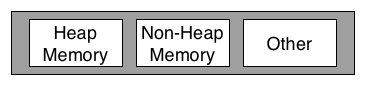
\includegraphics[width=2.7in]{image/Jvm_Heap.png}
    \caption{Java virtual machine memory structure.}
    \label{ref:heap_structure}
\end{figure}
The Heap Memory is the storage for Java objects, which occupies normally the largest part of JVM memory. The default Heap Memory size is 200 MB ({\bf -Xmx200m}) in Hadoop, by modifying this value can users specify memory space allocated to tasks.
In the runtime the total memory usage of the JVM may exceed the value specified in the command after "{\bf -Xmx}", this is because of the non-heap memory and other storage in JVM memory.
The Non-Heap Memory  is created at the JVM startup and store structures such as runtime constants, method data, the code for methods and constructors, and interned Strings.
There are also some other parts that might consume memory including JVM code itself, JVM internal structures, loaded profiler agent code and data, etc, which normally occupie a small portion of total JVM memory. 

\subsubsection{TaskMemoryManagerThread}
In addition to the execution of tasks, Hadoop also monitors these tasks and provides metrics reflecting their status for the purpose of rescheduling the killed ones.
In the Linux environment, TaskTrackers monitor tasks based on the following two conditions:  1) The memory usage of a specific task; 2) The total amount of memory usage of multiple tasks.
In the former situation, a task is killed and rescheduled by the TaskTracker if it fails either of the following two criteria:
i. Anytime when the current memory usage of a task exceeds two times of the value specified by {\bf mapred.cluster.max.map.memory.mb};
ii. The current memory usage of a task exceeds the value specified by {\bf mapred.cluster.max.map.memory.mb} for two consecutive periods of time (default is 5s). 
The first criteria considers the operation of fork(), which results in duplicated memory usages; the second criteria is applied to avoid the appearance of stragglers.
In the latter situation, tasks are killed by the TaskTracker if the following criteria is satisfied:
\begin{equation}
{\emph memInUsage} > {\emph maxMemAllowedForAllTasks} 
\end{equation}
where \emph {memInUsage} denotes the total memory in use of all the tasks scheduled by a specific TaskTracker and \emph {maxMemAllowedForAllTasks} denotes the total amount of memory allocated to it. The latter parameter can be calculated as following:
\begin{equation*}
\begin{aligned}
&{\emph maxMemAllowedForAllTasks} = \\
& \hspace {5pt} {\emph maxCurrMapTasks} \times {\emph mapSlotMemSizeOnTT} + \\
& \hspace {5pt} {\emph maxCurrReduceTasks} \times {\emph reduceSlotSizeMemOnTT}
\end{aligned}
\end{equation*}
In the above equation, \emph {maxCurrMapTasks} (specified by {\bf mapred.tasktracker.map.tasks.maximum} in the code) denotes the number of map slots allocated to that TaskTracker and \emph {mapSlotMemSizeOnTT}, which is specified by {\bf mapred.cluster.map.memory.mb}, denotes the memory size of a map slot. 
For reduce tasks, the situations are similar except that the parameters applied are different.
All tasks are killed by TaskTracker in the reverse order of scheduled time, \emph{i.e.}, recent tasks are killed until equation (1) fails. 
\subsubsection{Excessive Slots}
There is another case when Hadoop jobs may encounter memory failures: the virtual memory allocation request is under the limit specified by JVM, but the total value exceeds the amount of actual physical memory in the machine where TaskTracker is running.
This case can happen due to inappropriate settings on the number of slots (default value is 2) allocated to the TaskTracker. Consider the case illustrated in Figure \ref{ref:excessive_slots}.
\begin{figure}[ht]
  \centering
    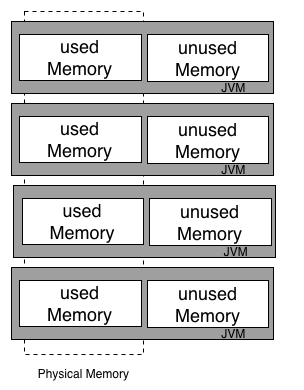
\includegraphics[width=2.1in]{image/excessive_Slots.png}
    \caption{Excessive number of slots}
    \label{ref:excessive_slots}
\end{figure}
\par
Suppose the physical memory space is 800 MB, the JVM heap size is 300 MB and one TaskTracker is allocated with 4 slots. Hadoop would run smoothly if the total memory consumed in the four JVMs is under 800 MB, but once the total amount of memory consumed exceeds the physical memory space, errors would occur and Hadoop would have to kill the running tasks to reduce the amount of memory occupied, or just abort the whole process.
\par
With appropriate parameters tuning, users can better manage the memory consumed by tasks, and the JVM memory space can be fully utilized to avoid potential memory-related bugs existing in users' Hadoop programs.

\subsection{Related Work}
Even though Hadoop has its own monitoring system on each component, including the website on JobTracker to check the running status of each MapReduce job and the website on the Namenode to check the usage of Hadoop File System (HDFS), the information posted on these pages is always not enough for either naive or experienced users.
For naive users, they merely get the log description showing the failed status of their jobs without specific reasons; For experienced users who need to know more about the whole pipeline performance information involved with a bunch of jobs, the default monitoring system is not enough either.
With the popularity of complex pipeline MapReduce jobs, companies like LinkedIn, Hortonworks develop their own fine-grained monitor frameworks for Hadoop based on traditional monitoring frameworks for cluster nodes metrics.\par
Ganglia\cite{massie2004ganglia}, developed from the project named Millennium in UC Berkeley, is a scalable distributed monitoring tool for high performance computing systems, which naturally integrates with Hadoop.
Ganglia follows the master/slave infrastructure, running a Ganglia monitoring daemon (Gmond) on each node in the cluster that needs to be monitored.
Gmond collects metric information on this node such as metrics of CPU,memory, etc, and sends it to Ganglia Meta Daemon (Gmetad) running on the master monitoring node of the cluster via XML over TCP periodically.
The Gmetad process runs on the master monitoring node (may not be the master of a cluster) to collect the metrics from distributed Gmond processes and Ganglia has its own default PHP web front end to show these metrics with dashboards.
%Gmond is a multi-threaded daemon which monitors changes in host state, announce the metrics data in Unicasting or Multicasting way. Hadoop has support of integration with Ganglia


Nagios (Nagios Ain’t Goona Insist On Saintood) \cite{josephsen2007building} is an open-source monitoring system that has great freedom and flexibility. 
The core of Nagios is concise, but it can be extended with specific plug-ins for different requirements, including plug-ins implemented by the users themselves.
These plug-ins run on distributed nodes to monitor the their status and send metrics to the core. 
The advantages of Nagios is that it provides a bunch of alerts mechanism that can notify the administrator when there is a problem in the system.
\par
Chukwa\cite{boulon2008chukwa} is a subproject of Hadoop, which is a distributed log analysis monitoring system. 
Different from Ganglia or Nagios, which are real-time monitoring systems, Chukwa is a batch log analysis system with the ability of processing large data brought by Hadoop.
Chukwa provides a full stack solution for large scale log data including data collection, storage, analysis and dashboard display.
Chukwa also deploys an agent running on each node to monitor metrics status on that node and the "Chukwa Collector" takes responsibility to collect these metrics data from distributed agents. 
After classifying, sorting, de-duplicating and combining, those logs will be directly written to HDFS or HBase (the open-source version of Google Big Table\cite{chang2008bigtable}) which can be used as the input source for MapReduce analysis jobs, then the results of the analysis are displayed through websites.
Users can check the running status of MapReduce jobs including the running time, resource consumption, when the failure happens and where the bottleneck is of the whole pipeline which largely enrich the monitoring functionality.
\par
SequenceIQ\cite{http://sequenceiq.com} is a real-time distributed monitoring system built directly atop InfluxDB and Grafana which provides comprehensive analysis on various metrics such as CPU, memory, network usage, etc.
InfluxDB\cite{http://influxdb.com} is a time series, metrics and analytics distributed database that can be used as part of the monitoring system due to its specific design for storing metrics data and support for abundant SQL queries for analysis.
Each node in the cluster can insert metrics data into InfluxDB, users do not need to care about the distributed messages and data transferring; instead they just need to use database functions to update the metrics.
Grafana\cite{http://grafana.org} is a well-designed and easy-to-use website development tool which integrates dashboards with analytics. Grafana provides rich graphing, mixed styling which render it a powerful frontend analysis tool.
\par

Cloudera Manager\cite{http://www.cloudera.com} is the first job management application for Hadoop clusters in the industry, which is also a commercial product.
It is designed to make the administration of enterprise data hub at any scale simple and straightforward, which provides users cluster-wide, real-time views of nodes/jobs running status, incorporating a full range of reporting and diagnostic tools to help users optimize the Hadoop job performance.

Ambri\cite{http://hortonworks.com/hadoop/ambari} developed by Hortonworks is an open-source version of Cloudera Manager which can be used to monitor the status of Hadoop jobs.
Ambri adopts Ganglia to collect metrics and Nagios to support the alert system, based on which users can check the status of Hadoop core as well as HBase and Hive.
For the purpose of integrating with existing administration tools, Ambri exposes the monitoring metrics through RESTful API.
\par
White Elephant\cite{http://data.linkedin.com/opensource/white-elephant}, developed by LinkedIn, is an open sourced Hadoop log aggregating tool and dashboard which enables visualization of Hadoop cluster utilization across users. 
White Elephant runs a daemon on each node in the cluster to periodically collect the log data, then it runs a sequence of MapReduce jobs to compute aggregate statistics. In the end, White Elephant applies a viewer application to display the metrics with dashboard.
\par
The difference between our system and Chukwa and White Elephant is that we use real-time metrics collected from Ganglia instead of the logs in each node.
Unlike Cloudera Manager, Ambri, and White Elephant which provide a general monitoring system, our system focuses on memory by providing fine-grained monitoring on task level and event detection for memory usages. It also provides the parameter description for users to modify to improve the performance of their Hadoop programs.


